% !TeX root = 00_Vorlage.tex
% !TeX spellcheck = de_DE
\chapter{Ergebnisse}
\label{sec:ergebnisse}

Im folgenden Abschnitt werden die Ergebnisse der Massenbestimmungen und der anschließenden Versuchen mit einer und mehrerer Federn. Alle Fehlerangaben beziehen sich auf statistische Fehler; Systematische werden gegebenenfalls separat diskutiert. 

\section{Massenbestimmung}
Die Masse des Pendelkörpers wurde über eine simultane Kraft- und Beschleunigungsmessung und Newtons Axiom \autoref{eqn:newt} bestimmt. In \autoref{fig:mass} sind die Messdaten auf die Zeit aufgetragen. In der ersten halben Sekunde befindet sich das Gerät am Tisch in Ruhe und ab \( t = 4 \unit{s} \) ist das IOLab komplett in der Luft. Ab diesem Zeitpunkt wird eine Konstante an die Messdaten angepasst. 

\begin{figure}[H]
	\centering
	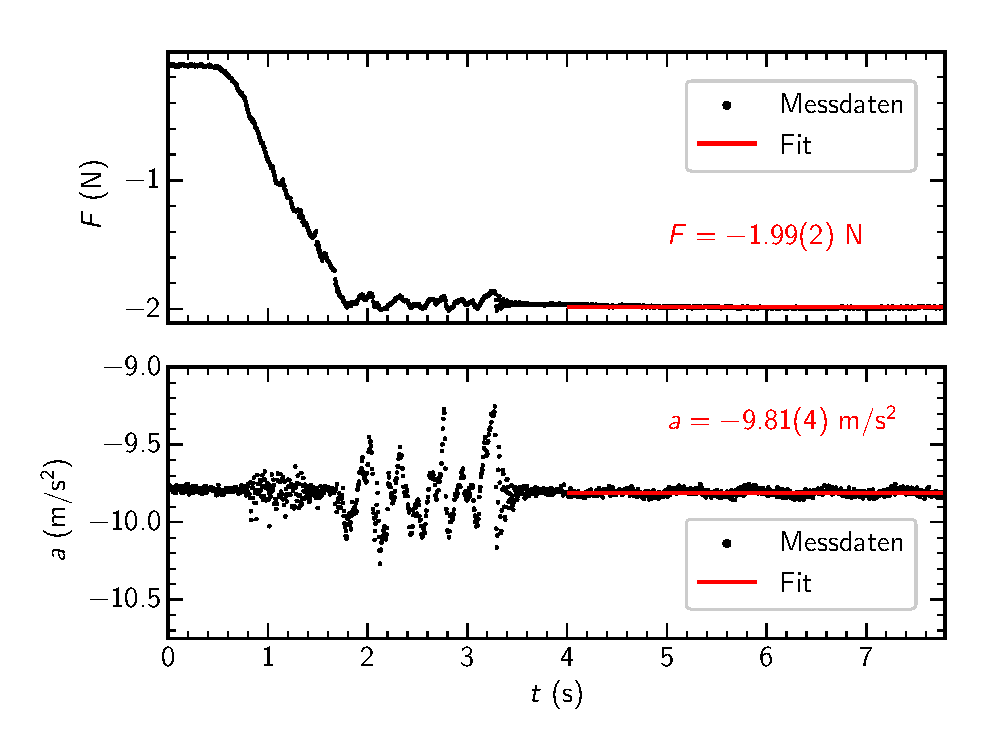
\includegraphics[width=\textwidth]{mass.eps}
	\caption{Vom oben nach unten sind Kraft \( F \) und Beschleunigung \( a \) aufgetragen. Die Fehlerbalken der Daten sind zu klein, um sie auszumachen und werden daher nicht eingetragen. Die zwei Grafiken teilen sich die horizontale Achse. Zudem sind in Rot Geraden von \( t = 4 \unit{s} \) bis \( t = 8 \unit{s} \) angepasst.}
	\label{fig:mass}
\end{figure}

Der bestimmte Wert mit Fehler ist sowohl in der Abbildung, als auch in \autoref{table:1} zu sehen. Die Unsicherheit wurde auf die Standardabweichung der Daten gesetzt, da dann (per Definition) Zwei Drittel der Daten innerhalb des \( 1\sigma \) Intervalls liegen.

\begin{center}
	\captionof{table}{Gemessene Beschleunigung und Kraft und die daraus errechnete Masse der drei Versuche.}
	\begin{tabular}{@{\extracolsep{5mm}} 
			r
			S[table-format=1.2(1)]
			S[table-format=1.2(1)]
			S[table-format=1.2(1)]
		}
		\toprule
		\makecell[t]{}
		&   {\makecell[t]{Versuch 1}}
		&   {\makecell[t]{Versuch 2}}
		&   {\makecell[t]{Versuch 3}}\\
		\midrule
		\( a \unit{(\a)} \) & -9.81(4) & -9.73(6) & -9.81(8) \\
		\( F  \unit{(N)} \) & -1.99(2) & -2.78(2) & -3.93(7) \\
		\( m \unit{(kg)} \) & 0.202(2) & 0.286(3) & 0.400(7) \\
		\bottomrule
	\end{tabular}
	\label{table:1}
\end{center}

\section{Federpendel 1}
Für die Analyse der Oszillation wurde der Beschleunigungssensor verwendet, da dieser eine höhere Auflösung hat als der Kraftsensor. In \autoref{fig:sine} sind die Schwingungsdaten der zweiten Masse dargestellt. Links sind die ersten fünf Sekunden mit „schönen” Schwingungen zu sehen, während rechts die letzten Sekunden der Messung aufgetragen sind. In rot wurde eine Sinuskurve der Form \( f(x) = A\sin(\omega x + \phi) + d \) an die gesamten Messdaten von \( t = 4 \unit{s} \) bis \( t = 27 \unit{s} \) angepasst. 
	
\begin{figure}[H]
	\centering
	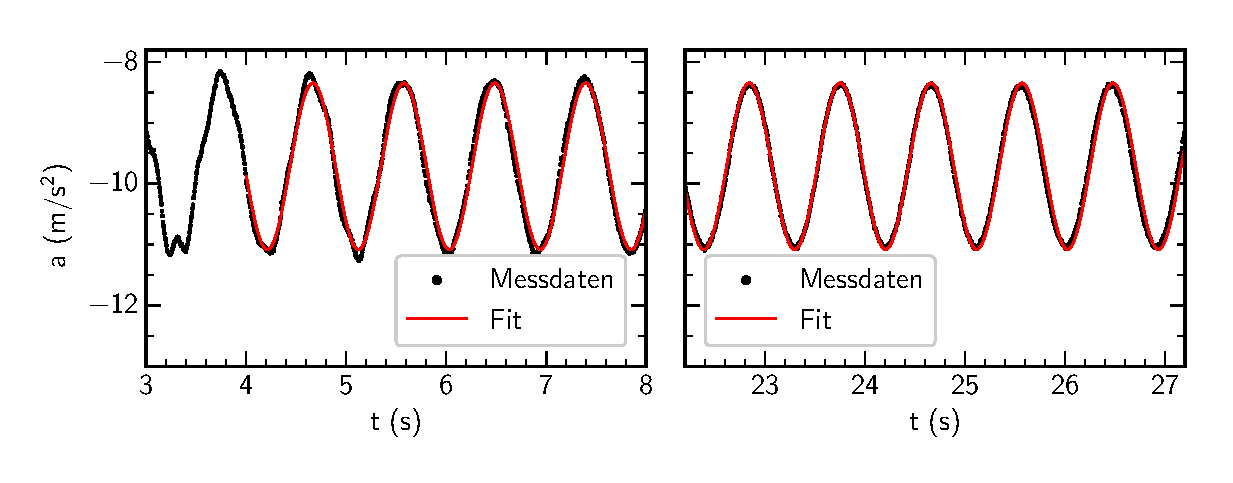
\includegraphics[width=\textwidth]{Feder1.eps}
	\caption{Die Beschleunigung wurde auf die Zeit aufgetragen und eine durchgehende Sinuskurve in Rot wurde an die Daten ab \( t = 4 \unit{s} \) (bis \( t = 27 \unit{s} \)) angepasst. Dargestellt werden aber nur ersten 5 Sekunden (links) beziehungsweise letzten 5 Sekunden (rechts). Die Fehlerbalken der Daten sind zu klein, um sie auszumachen und werden daher nicht eingetragen.}
	\label{fig:sine}
\end{figure}
	
Aus dem Fit lässt sich direkt die Winkelfrequenz \( \omega \) herauslesen. Aus dieser kann man wiederum mit \autoref{eqn:T} die Schwingungsdauer berechnen. In \autoref{table:2} sind charakteristische Eigenschaften der Schwingung, wie die Kreisfrequenz oder die Masse, eingetragen. 
	
\begin{center}
	\captionof{table}{Gemessene Masse, Schwingungsdauer, Winkelfrequenz und Federkonstante der drei Versuche.}
	\begin{tabular}{@{\extracolsep{5mm}} 
			r
			S[table-format=1.3(1)]
			S[table-format=1.3(1)]
			S[table-format=1.3(1)]
		}
		\toprule
		\makecell[t]{}
		&   {\makecell[t]{Versuch 1}}
		&   {\makecell[t]{Versuch 2}}
		&   {\makecell[t]{Versuch 3}}\\
		\midrule
		\( m \unit{(kg)}\) & 0.202(2) & 0.286(3) & 0.400(7) \\
		\( \sqrt{1/m} \unit{(\sqrt{1/kg})} \) & 2.223(10) & 1.8698(99) & 1.580(15) \\
		\( T \unit{(s)} \) & 0.749(2) & 0.909(5) & 1.063(10) \\
		$\omega \unit{(1/s)}$ & 8.39(2) & 6.91(4) & 5.91(6) \\
		\( k \unit{(N/m)} \) & 14.24(15) & 13.7(2) & 14.0(4) \\
		\bottomrule
	\end{tabular}
	\label{table:2}
\end{center}

Das Modell des harmonischen Oszillators (Siehe \autoref{eqn:harm}) stellt einen linearen Zusammenhang zwischen \( \omega \) und der Wurzel des Kehrwerts der Masse her. 